\documentclass{BeamerTemplate}
\title{Module 8 - Estimation par intervalles de confiance}
\subtitle{STT-1000 Probabilités et statistique}

\usepackage{adjustbox}


\begin{document}
\AtBeginSection{\frame{\sectionpage}}

\begin{frame}

\titlepage

\end{frame}

\section{Introduction}

\begin{frame}{Introduction: estimation ponctuelle imparfaite}

Un échantillon donne lieu à UNE estimation du paramètre. Quelle confiance peut-on avoir en cette estimation?\\
{\small \it Ci-dessous, chaque échantillon $X_1,...X_{25}$ provient d'une $\mathcal{N}(15,\,16)$.}
\vspace{0.5cm}

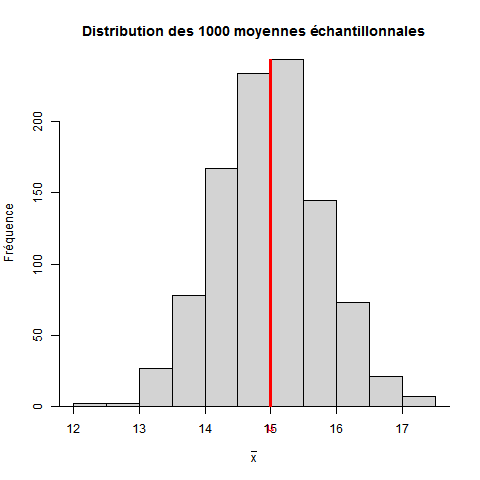
\includegraphics[width=5.0cm]{moy1000.png}
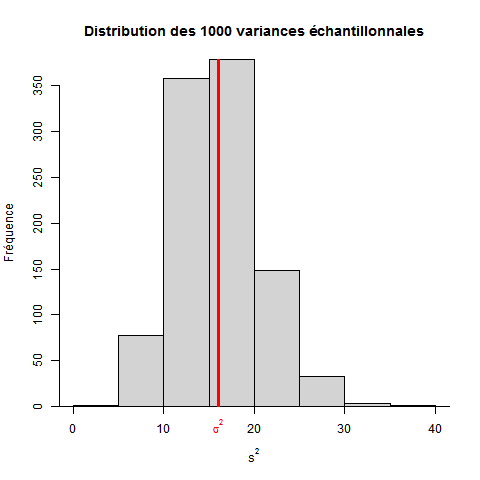
\includegraphics[width=5.0cm]{var1000.png}

\end{frame}


\begin{frame}[t]
Dans l'histogramme de gauche (page précédente),\\
les 1000 valeurs de $\overline x$ pourraient servir d'estimation pour $\mu$.
\bigskip


Dans cette situation, environ combien d'estimations sont distantes de $\mu$ d'au moins 1,5 tonnes?

\vspace{2cm}

\end{frame}

\begin{frame}[t]
 \frametitle{Concept d'estimation par intervalle de confiance}

Un intervalle de confiance :
\medskip

    \begin{itemize}\itemsep8mm
    \item complète l'estimation ponctuelle en l'entourant d'une \alerter{marge d'erreur}.

    \item donne une idée de la précision obtenue avec l'échantillon.

    \item est associé à un \alerter{niveau de confiance} (probabilité que l'intervalle contienne la vraie valeur du paramètre).
    \end{itemize}

\end{frame}


\begin{frame}[t]
 \frametitle{Définition formelle}
 \begin{itemize}
\item $X_1,\ldots,X_n$:  échantillon aléatoire de taille $n$;
\item $\theta$:  paramètre d'intér\^et (comme $\mu$ ou $\sigma^2$);
 \end{itemize}
 
 \begin{Boite}{Intervalle de confiance de niveau $1-\alpha$ pour un paramètre $\theta$}
 Deux statistiques  $[C_1, C_2]$ calculées à partir de l'échantillon telles que  \alert{$$P(C_1\le \theta\le C_2)=1-\alpha$$}
 \end{Boite}

 \medskip
 \uncover<2->{
 \begin{itemize}
\item $1-\alpha$: niveau de confiance de l'intervalle \\(fixé arbitrairement par le chercheur).
\item Souvent $1-\alpha=0,95$. Parfois $1-\alpha=0,90$ ou $0,99$ ou autre.
 \end{itemize}
 }
\end{frame}
\begin{frame}[t]
 \frametitle{Plusieurs intervalles de confiance }

\begin{minipage}[b]{3cm}

\includegraphics[width=2.8cm]{quote.png}
\end{minipage}
\begin{minipage}[b]{7.5cm}
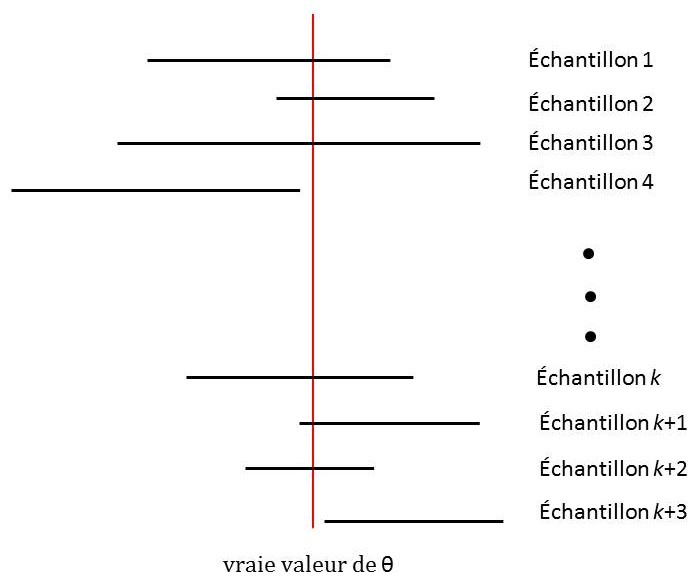
\includegraphics[width=7.5cm]{interpret-ic2.jpg}
\end{minipage}

\end{frame}
\begin{frame}{Rappel sur les lois échantillonnales}

 Lorsque $X_1, ..., X_n$ i.i.d. $N(\mu, \sigma^2)$, on connaît les lois échantillonnales des statistiques suivantes:

\begin{center}
{\renewcommand{\arraystretch}{2.5}
\begin{tabular}{|c|l|c|c|}
\hline Statistique & Loi échantillonnale &Espérance& Variance \\[-0.15cm]
\hline \hline
$\displaystyle Z=\frac{\overline X -\mu }{\sigma/\sqrt{n}}$ &&& \\\hline
$\displaystyle T=\frac{\overline X -\mu }{S/\sqrt{n}}$ &&&\\\hline
$\displaystyle U=\frac{(n-1)S^2 }{\sigma^2}$ &&&\\\hline
\end{tabular}
}
\end{center}

 \vspace{1cm}

\end{frame}

\begin{frame}[t]{5 cas étudiés}

Nous construirons 5 intervalles de confiance:
\vspace{0.5cm}

\begin{tabular}{|c|c|l|}
  \hline
  Cas&Paramètre & Situation \\\hline
&&\\[-0.3cm]
1&  $\mu$ & $X_1, ..., X_n\;\sim\;N(\mu, \, \sigma^2)$ avec $\sigma^2$ connue \\
&&\\
2&  $\mu$ & $X_1, ..., X_n\;\sim\;N(\mu, \, \sigma^2)$ avec $\sigma^2$ inconnue  \\
&&\\
3&  $\mu$ & $X_1, ..., X_n\;\sim\;$ loi inconnue, mais $n$ est grand  \\[0.2cm]\hline
&&\\[-0.3cm]
4&  $p$ & $X_1, ..., X_n \sim \text{Bernoulli}(p)$ avec $n$ assez grand  \\[0.2cm]\hline
&&\\[-0.3cm]
5&  $\sigma^2$ & $X_1, ..., X_n\;\sim\;N(\mu, \, \sigma^2)$ \\[0.2cm]\hline

\end{tabular}
\end{frame}

\section{Intervalles de confiance pour la moyenne}


\begin{frame}[t]
 \frametitle{Cas 1 pour $\mu$: loi normale, variance CONNUE}

\small
\begin{itemize} \itemsep1mm
\item {\color{blue}{On suppose que $X_1,\ldots,X_n$ i.i.d. loi $N(\mu,\sigma^2)$, \\
o\`u $\sigma^2$ est  une valeur connue}.}% et $\mu$ est le paramètre d'intér\^et.
\item On déduit que $\overline X\;\sim\;N\left(\mu,\displaystyle\frac{\sigma^2}{n}\right)$, donc que    $\displaystyle Z=\frac{\overline X-\mu}{\sigma/\sqrt{n}}\;\sim\;N(0,1)$
\item Soit $z_{\alpha/2}$, la valeur telle que $P(Z>z_{\alpha/2})=\alpha/2$. On a donc que\\
\end{itemize}

\begin{minipage}{5cm}{
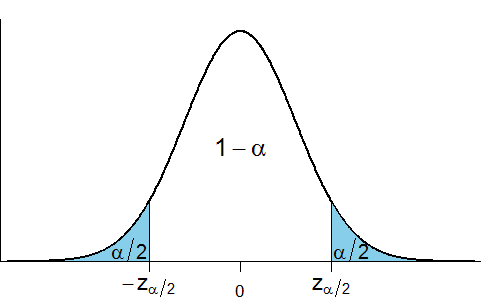
\includegraphics[width=6cm]{N.png}}
\end{minipage}
\begin{minipage}[b]{5cm}{
$P(\,-z_{\alpha/2}\;\le \;Z\;\le \;z_{\alpha/2}\,)=1-\alpha$.

\vspace{1cm}}
\end{minipage}
\end{frame}


\begin{frame}[t]
 \frametitle{Cas 1 pour $\mu$: loi normale, variance connue}

\begin{itemize} \itemsep3mm
\item On cherche $[C_1, C_2]$ tels que $P(C_1\le \alert{\mu} \le C_2)=1-\alpha$
\item On sait que $P\left(\,-z_{\alpha/2}\;\le \;\dfrac{\overline X - \mu}{\sigma/\sqrt{n}}\;\le \;z_{\alpha/2}\,\right)=1-\alpha$
\end{itemize}

\end{frame}

\begin{frame}[t] \frametitle{Exemple 1 }

 {\small
 Soit $X$, le diamètre (en cm)  des disques de frein  produits par une machine, o\`u $X\sim N(\mu,\, 0,0009)$.  On choisit un échantillon de 9 disques  au hasard et on calcule un diamètre moyen de $12,05$ cm.

 \vspace{3mm}

 \alerter{a)} Donnez un intervalle de confiance de niveau 95\% pour $\mu$. 
 }
\end{frame}

\begin{frame}[t]
Déterminez si les énoncés suivants (liés à l'exemple 1) sont vrais ou faux.

\begin{itemize} \itemsep2mm
\item 95\% des disques de cette compagnie ont un diamètre entre 12,03 et 12,07 cm.
\item 95\% des intervalles calculés avec cette formule (à partir d'échantillons différents) contiendraient le vrai diamètre moyen.
\item On a confiance à 95\% que la vraie valeur de $\mu$ est comprise entre 12,03 et 12,07 cm.
\item Si on prenait un nouvel échantillon de taille $n=9$, la probabilité que sa moyenne $\overline X$ soit entre 12,03 et 12,07 cm est de 95\%.
\end{itemize}

\end{frame}

\begin{frame}[t]{Exemple 1: taille d'échantillon}

 {\small
 \alerter{b)} Quelle taille d'échantillon devrait-on collecter pour que la marge d'erreur sur l'estimation du diamètre moyen ne dépasse pas 0,01 cm, si on conserve un niveau de confiance de 95\% ?
}

\end{frame}


\subsection{Loi normale, variance inconnue}

\begin{frame}[t]
 \frametitle{Cas 2 pour $\mu$: loi normale, variance INCONNUE}

 \begin{itemize} \itemsep1mm
\item {\color{blue}{On suppose que $X_1,\ldots,X_n$ i.i.d. loi $N(\mu,\sigma^2)$, \\
o\`u $\sigma^2$ est  une valeur inconnue, donc à estimer par $S^2$}.}% et $\mu$ est le paramètre d'intér\^et.
\item On déduit que $\overline X\;\sim\;N\left(\mu,\displaystyle\frac{\sigma^2}{n}\right)$, donc $T=\dfrac{\overline X-\mu}{S/\sqrt{n}}\;\sim\;t_{n-1}$
\item Soit $t_{\alpha/2; n-1}$, la valeur telle que $P(T>t_{\alpha/2;\, n-1})=\alpha/2$. Ainsi,\\
\end{itemize}

\begin{minipage}{4.8cm}{

\includegraphics[width=6cm]{t.png}}
\end{minipage}
\begin{minipage}[b]{5.8cm}{
$P(-t_{\alpha/2;\, n-1}\le T\le t_{\alpha/2;\,n-1})=1-\alpha$.

\vspace{1cm}}
\end{minipage}

% \centerline{\includegraphics[height=3.3cm]{talpha-student.jpg}}

\end{frame}

\begin{frame}[t]
 \frametitle{Cas 2 pour $\mu$: loi normale, variance inconnue}

 \begin{itemize} \itemsep3mm
\item On cherche $[C_1, C_2]$ tels que $P(C_1\le \alert{\mu} \le C_2)=1-\alpha$
\item On sait que $P\left(\,-t_{\alpha/2;\, n-1}\;\le \;\dfrac{\overline X - \mu}{S/\sqrt{n}}\;\le \;t_{\alpha/2;\, n-1}\,\right)=1-\alpha$
\end{itemize}

%$\frac{\bar{X}-\mu}{S/\sqrt{n}}\sim t_{n-1}\Rightarrow$
\end{frame}

\begin{frame}[t]
 \frametitle{Exemple 2}
 Retournons à l'exemple des disques. Supposons que $\sigma^2$ n'était pas
 connue et qu'on l'estime par la variance échantil\-lonnale des 9 diamètres observés, soit $s^2= 0,0009 \;\text{cm}^2$.

 \vspace{3mm}

 Donnez un intervalle de confiance à 95\% pour $\mu$. Comparez-le avec l'intervalle oBoitenu en supposant la variance connue.
\end{frame}

\subsection{Loi de $X_1,\ldots,X_n$ inconnue, mais $n$ grand}

\begin{frame}[t]
 \frametitle{Cas 3 pour $\mu$: loi inconnue, n grand}

 \begin{itemize} \itemsep3mm
\item {\color{blue}{On suppose que $X_1,\ldots,X_n$ sont i.i.d. d'une loi inconnue. }}% et $\mu$ est le paramètre d'intér\^et.
\item  Peut-on construire des intervalles de confiance?

 \item <2->L'idée: utiliser le \alerter{théorème  central limite } et le fait  que pour $n$ grand :%(dans la pratique on recommande $n\ge 30$):

 \vspace{4mm}
  $s^2\simeq \sigma^2$ et $\overline{X}\approx N(\mu,s^2/n)\Rightarrow$
\vspace{1cm}
\item <2->
 Si $n$ est grand, on peut construire des intervalles de confiance dont le niveau sera \alerter{approximativement}  du niveau désiré.
\end{itemize}
\end{frame}

\begin{frame}[t]
 \frametitle{Cas 3 pour $\mu$: loi inconnue, n grand}

 \begin{itemize} \itemsep3mm
\item On cherche $[C_1, C_2]$ tels que $P(C_1\le \alerter{\mu} \le C_2)=1-\alpha$
\item On sait que $P\left(\,-z_{\alpha/2 }\;\le \;\dfrac{\overline X - \mu}{S/\sqrt{n}}\;\le \;z_{\alpha/2 }\,\right)\alerter{\approx} 1-\alpha$
    \vspace{7mm}
\item On déduit que $P\left(\overline X \,-\,z_{\alpha/2 } \dfrac{S}{\sqrt{n}}\;\le \;  \mu\;\le \overline X \,+\,z_{\alpha/2 }\dfrac{S}{\sqrt{n}}\,\right)\alerter{\approx} 1-\alpha$
\end{itemize}
% $s^2\simeq \sigma^2$ et $\bar{X}\approx N(\mu,s^2/n)\Rightarrow$
\end{frame}

\begin{frame}[t]
 \frametitle{Exemple 3}

 {\small
 Pour estimer le salaire moyen annuel de jeunes diplômés dans un certain domaine, on  a prélevé un échantillon de taille $n = 100$ et oBoitenu  $\overline{x}=34~224\,\$$ et $s=4~668\,\$$.\\

 Donnez un intervalle de confiance de niveau 90\% pour le salaire moyen annuel des  jeunes diplômés dans ce domaine.}



\end{frame}


\begin{frame}[t]{La marge d'erreur et l'erreur-type}
Les trois intervalles de confiance pour $\mu$ sont symétriques:

$$\begin{array}{cccc}
\overline X &\pm & \multicolumn{2}{c}{\alerter{\text{marge d'erreur}}}\\[6mm]
\overline X &\pm & \text{quantile}\;\times&\text{\color{green}{erreur-type}}
\end{array}$$

\vspace{3cm}
{\color{blue}{Longueur}} de l'intervalle$ = 2\times $ marge d'erreur

\end{frame}

\begin{frame}[t]%{Événements mutuellement exclusifs}

\centerline{\LARGE \bf \alert{QUIZ !}}
Déterminez si les énoncés suivants sont vrais ou faux.
\vspace{0.3cm}

La marge d'erreur d'un IC sur la moyenne $\mu$ augmente \\(donc la précision diminue) si:
\vspace{0.3cm}

\begin{itemize}\itemsep1cm
  \item la variabilité des mesures augmente.
  \item la taille d'échantillon augmente.
  \item le niveau de confiance augmente.
\end{itemize}

\end{frame}

%%%%%%%%%%%%%%%%%%%%%%%%%%%%%%%%%%%%%%%%%%%%%%%%%%%%%%%%%%%%%%%%%%%%%%%%%%%%%%%%%%%%%%%%%%%%%%%%%%%%%%%%%%%%%%%%%%%%%%%%%%%
\section{Intervalle de confiance pour une proportion}

\begin{frame}[t]{Cas 4 pour une proportion}


 \begin{itemize} \itemsep1mm
\item {\color{blue}{On suppose que $X_1,\hdots,X_n$ i.i.d. loi Bernoulli$(p)$,
où $p$ inconnue et où $n\geq 30$}.}
\item L'estimateur ponctuel pour $p$ est $\hat{p} =\displaystyle \frac{1}{n}\sum_{i=1}^n X_i$
\item Par le TCL, nous savons que $\hat{p}\approx \mathcal{N}(p, \frac{p(1-p)}{n})$ et donc $$\frac{\hat{p}-p}{\sqrt{\frac{p(1-p)}{n}}}\approx \mathcal{N}(0,1)$$
\end{itemize}
Ainsi,
$$P\left(-z_{\alpha/2}\leq \frac{\hat{p}-p}{\sqrt{\frac{p(1-p)}{n}}} \leq z_{\alpha/2} \right)\approx 1-\alpha$$
\end{frame}
\begin{frame}[t]{Cas 4 pour une proportion}
On en déduit donc l'intervalle de confiance de niveau approximatif $(1-\alpha)$:
$$P\left(\hat{p}-z_{\alpha/2}\sqrt{\frac{p(1-p)}{n}} \leq p \leq \hat{p}+z_{\alpha/2} \sqrt{\frac{p(1-p)}{n}} \right)\approx 1-\alpha$$
\pause
Mais il y a un problème.
\end{frame}

\section{Intervalles de confiance pour la variance}

\subsection{Loi normale}

\begin{frame}[t]
 \frametitle{Cas 5 pour $\sigma^2$: loi normale, $\mu$ et $\sigma^2$ inconnues}


 \begin{itemize} \itemsep1mm
\item {\color{blue}{On suppose que $X_1,\ldots,X_n$ i.i.d. loi $N(\mu,\sigma^2)$, \\
o\`u $\mu$ et $\sigma^2$ sont inconnues}.}% et $\mu$ est le paramètre d'intér\^et.
\item On sait que  $\displaystyle U=\frac{(n-1)\,S^2}{\sigma^2}\;\sim\;\chi^2_{n-1}$
\item Soit $\chi^2_{\alpha/2;\,n-1}$, la valeur telle que $P(U>\chi^2_{\alpha/2;\,n-1})=\alpha/2$. Ainsi,\\
\end{itemize}


\begin{minipage}{4.2cm}{
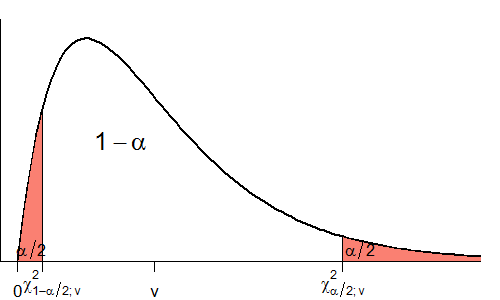
\includegraphics[width=6cm]{K.png}}
\end{minipage}
\begin{minipage}[b]{6.1cm}{
$P(\chi^2_{1-\alpha/2;\,n-1}\le U\le \chi^2_{\alpha/2;\,n-1})=1-\alpha$.

\vspace{1cm}}
\end{minipage}\end{frame}

\begin{frame}[t]
 \frametitle{Cas 5 pour $\sigma^2$: loi normale, $\mu$ et $\sigma^2$ inconnues}

 \begin{itemize} \itemsep3mm
\item On cherche $[C_1, C_2]$ tels que $P(C_1\le \alert{\sigma^2} \le C_2)=1-\alpha$
\item On sait que $P\left(\chi^2_{1-\alpha/2;\,n-1}\le \dfrac{(n-1)\,S^2}{\sigma^2}\le \chi^2_{\alpha/2;\,n-1}\right)=1-\alpha$
\end{itemize}

% {\small  On cherche deux v.a. $C_1$ et $C_2$ telles que $P[C_1\le\sigma^2\le C_2]=1-\alpha$. On sait  que $\frac{(n-1)S^2}{\sigma^2}\sim\chi^2_{n-1}\Rightarrow$}

\end{frame}

\begin{frame}[t]
 \frametitle{Intervalle pour l'écart-type $\sigma$}

  $P\left(C_1\le \sigma^2\le C_2\right)=1- \alpha $
  \bigskip

  est équivalent à
    \bigskip

  $P\left(\sqrt{C_1}\le \sqrt{\sigma^2}\le\sqrt{C_2}\right)=1 - \alpha $.
    \bigskip

  Pour avoir un IC($\sigma$), on prend la racine carrée des bornes de IC($\sigma^2$).

\end{frame}

\begin{frame}[t]
 \frametitle{Exemple 4}

 {\small
 On veut calibrer la machine qui fabrique les disques de frein pour qu'elle soit le plus stable possible. On veut d'abord estimer la variation du diamètre des disques produits, avec un intervalle de confiance  à 95\%.\\

 Un échantillon de taille 25  a donné une variance échantillonnale de $0,015$ cm$^2$.  On suppose que les diamètres sont i.i.d. de loi normale.}

\end{frame}

\begin{frame}{Bibliographie}
 	Ce document est rédigé avec Beamer ainsi qu'une classe .cls fourni par Jérôme Soucy. Les diapositives sont adaptées des diapositives créées par Thierry Duchesne et Emmanuelle Reny-Nolin pour le cours STT-1900. Les graphiques proviennent de ces mêmes diapositives.
 	\printbibliography
 	\vfill
 	\footnotesize Pour signaler une erreur dans ce document, veuillez écrire à l'adresse :~\href{mailto:julien.miron@mat.ulaval.ca}{julien.miron@mat.ulaval.ca}.
 \end{frame}

\end{document}

